\chapter{Výsledky studentské práce}

% Referenční skladby http://isophonics.net/about

\section{Návrh výsledného systému}

Návrh popisuje komplexní systém skládající se z několika částí, uživatelské rozhraní algoritmů pro získání pamrametrů hudební nahrávky a algoritmu generujícího SpectodaCode na základě získaných parametrů. V této kapitole je podrobně popsán návrh jednotlivých částí systému. 

\subsection{Uživatelské rozhraní}

Uživatelské rozhraní je reprezentováno webovou stránkou a je naprogramováno pomocí značkovacího jazyka \acs{HTML} spolu s formátováním v jazyce CSS. Funkčnosto webové stránky je zajištěna funkcemi jazyce JavaScript. Javascript také vytváří propojovací můstek pro komunikaci s vnistřním systémem v jazyce Python.

Jedná se o jednoduché webové rozhraní ve kterém uživatel nahraje hudební skladbu ve formátu .wav. Rozhranní obsahuje pole pro vložení cesty k hudební skladbě umožňující výběr ze souborů v uživatelově uložišti. Níže je posuvník s 4 základními hodnotami pro výběr nálady
\uv{mood}. Jedná se hodnoty \uv{chill}, \uv{hang out}, \uv{feeling happy} a \uv{dancing}, které jsou v tomto pořadí na posuvníku. Uživatel může pomocí posouvání posuvníku vybrat pro jakou náladu chce vytvořit animaci. Pod posuvníkem pro výběr nálady se nachází tlačítko pro spuštění procesu generování SpectodaCodu.
Poslední částí webového rozhraní je textové pole ve kterém se zobrazí vygenerovaný SpectodaCode.

 \begin{figure}[H]
    \centering
    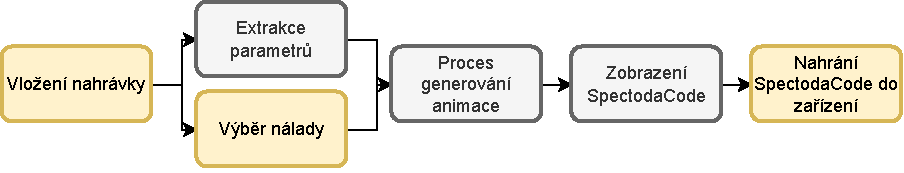
\includegraphics[width = 1\linewidth]{obrazky/User_interaction_diagram.pdf}
    \caption{Blokové schéma postupu uživatele webovou stránkou}
    \label{fig:User_interaction_diagram}
\end{figure}

Na blokovém schématu \ref{fig:User_interaction_diagram} je zobrazen proces postupu uživatele skrze webové rozhraní. 

\subsection{Parametry hudební nahrávky} \label{sec:Parametry_nahravky}

Systém popsaný v bodě \ref{sec:System_generovani_animaci} vyžaduje vstupní data o hudební nahrávce. Tyto data jsou rozdělena 7 odlišných objektů. Každý z těchto objektů představuje určitou vlastnost analyzované nahrávky. Tyto vlastnosti jsou získány pomocí technik popsaných v bodě \ref{sec:Exktrakce_vlastnosti_metody}. Jednotlivé vlastnosti a jejich datové struktury jsou shrnuty v následujících bodech.

\begin{description}
    \item[Detekce dob] představuje pole hodnot jehož délka je závislá na době trvání nahrávky. Jednotlivé hodnoty pak udávají časy hudební nahrávky, ve kterých se nacházejí doby.
    \item[Tempo skladby] je číslo typu float s jednotkou \acs{BPM} vyjadřující počet úderů za minutu. Hodnota BPM se vztahuje k počtu čtvrťových not za minutu. Vybraný algoritmus s knihovny Librosa ovšem nedetekuje jestli se jedná o noty čtvrťové. Postup zjištění tempa je popsán v bodě \ref{Librosa}.
    \item[Chromavektory] jsou získány v podobě pole jehož počet řádků udává 12 půltónů rozdělujících 1 oktávu. Délka pole je závislá na délce nahrávky a velikosti okna  při výpočtu \acs{STFT}. K matici chromavektorů je přidáno pole o stejné délce. Hondonty v poli udávají čas konce okna, ve kterém jsou počítány chroma vlastonsti. Tyto dvě proměnné jsou zadány jako parametry třídy s názvem $ChromaVector$ jehož struktura je zobrazena v blokovém schématu \ref{fig:ChromaVector_class_diagram}.

    \begin{figure}[H]
        \centering
        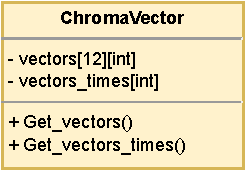
\includegraphics[width = 0.3\linewidth]{obrazky/UML_diagram_ChromaVector.pdf}
        \caption{Struktura třídy $ChromaVector$}
        \label{fig:ChromaVector_class_diagram}
    \end{figure}

    \item[Efektivní hodnota signálu] je zapsána třídou $Loudness$ obsahující dva atributy. Prvním z nich je pole $rms$ jehož délka je závislá na délce signálu a obsahuje efektivní hodnoty signálu v časech uložených v druhém atributu. Druhý atribut $times$ je pole o stéjné délce jako pole s hodnoty rms a obsahuje časy skladby ve kterých je hodnota rms počítána. 
    
    \begin{figure}[H]
        \centering
        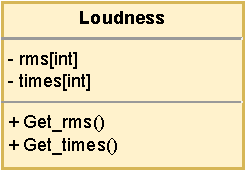
\includegraphics[width = 0.3\linewidth]{obrazky/UML_diagram_Loudness.pdf}
        \caption{Struktura třídy $Loudness$}
        \label{fig:Loudness_class_diagram}
    \end{figure}

    \item[Segmentace] je zapsána jako pole objektů tířdy $Segment$. Tato třída obshahuje 3 atributy $type$, $start\_time$ a $end\_time$. Argument $type$ obsahuje statickou hodnotu označující o jakou část skladby se jedná. Tyto hodnoty jsou vypsány v úryvku kódu \ref{code:song_segments_variables}.
    Argumenty $start\_time$ a $end\_time$ označují začátek a konec segmentu v nahrávce. 

    \begin{figure}[H]
        \centering
        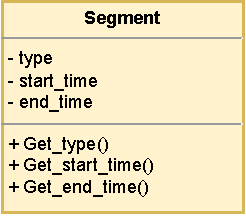
\includegraphics[width = 0.3\linewidth]{obrazky/UML_diagram_Segment.pdf}
        \caption{Struktura třídy $Segment$}
        \label{fig:Loudness_Segment_diagram}
    \end{figure}
    \begin{lstlisting} [
        caption = {Hodnoty proměnné $type$},
        captionpos=b,
        label = {code:song_segments_variables}]
        # Song segments variables
        SILENT      = 0
        REFRAIN     = 1
        STROPHE     = 2
        BRIDGE      = 3
    \end{lstlisting}

    \item[Žánr] představuju proměnou $genre$ typu short vekteré je zapsáno číslo označující žánr skladby. Statické hodnoty žánrů jsou zapsány v úryvku kódu \ref{code:song_genre_variables}.
    \begin{lstlisting} [
        caption = {Hodnoty proměnné $genre$},
        captionpos=b,
        label = {code:song_genre_variables}]
        # Song genre variables
        CLASSIC     = 0
        FOLK        = 1
        POP         = 2
        ROCK        = 3
        METAL       = 4
        ELECTRONIC  = 5
    \end{lstlisting}
    \item[Nálada] představuje proměnou $mood$ typu float s přednastavenými statickými hodnotami zobrazenými v části kódu \ref{code:song_mood_variables}. Nálada může být i v rozmezí přednastavencýh hodnot. V tomto případě je výsledná hodnot lineráně závislá na vzdálenosti od přednastavených hodnot. 
    \begin{lstlisting}[
        caption = {Hodnoty proměnné $mood$},
        captionpos=b,
        label = {code:song_mood_variables}]
        # Song mood variables
        CHILL       = 0
        HANG_OUT    = 1
        HAPPY       = 2
        DANCING     = 3
    \end{lstlisting}
    
\end{description}

\subsection{Systém pro generování animací} \label{sec:System_generovani_animaci}

Systém pro generování animací představuje nejduležitější část práce. Jeho struktura udává vizuální kvalitu animací a schopnost přizpůsobit se daným skladbám růtzných žánrů. V této kapitole je popsána základní struktura systému. 

První částí systému je vstupní rozhraní, ve kterém jsou přijímány data obsahující paramery o hudební nahrávce. Struktura přijímaných dat je popsána v budě \ref{sec:Parametry_nahravky}. Každý ze zmíněných parametrů plňí důležitou funkci v rozhodovacím procesu skládání bloků animace. Níže jsou popsány rozhodovací funkce pro jednotlivé parametry.

\begin{description}
    \item[Žánr a nálada] jsou používány pro výběr vhodného balíčku animací. Tyto balíčky jsou nazývány datasety a jejich datová struktu je popsána v bodě \ref{sec:Database_structure}. Źánr i nálada jsou zaznamenány jako předdefinovaná celočíslená hodnota. Postup výběru datasetu je následující. Každý dataset obsahuje seznam žánrů pro který je vhodný. Na základě proměnné $genre$ dochází k výběru všech datasetůch vhodných pro daný žánr. Následně na základě proměnné $mood$ ve které je uložená nálada je vabráno 5 datasetů s nejbližší hodnotou $mood\_characteristic$.
    
    \begin{figure}[H]
        \centering
        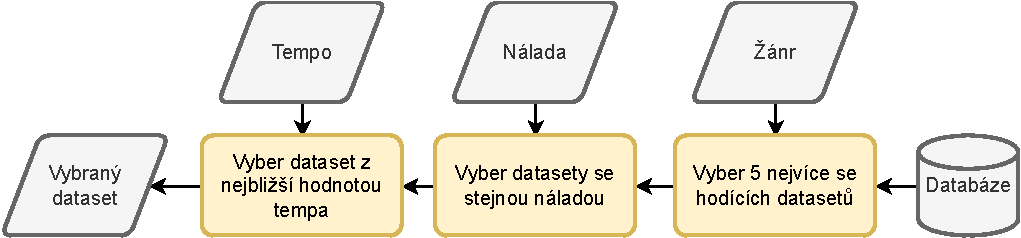
\includegraphics[width = 1\linewidth]{obrazky/Dataset_selection_diagram.pdf}
        \caption{Blokový diagram výběru datasetu.}
        \label{fig:Dataset_selection_diagram}
    \end{figure}

    \item[Tempo skladby] je posledním parametrem při výběru vhodného datasetu. 
    Hodnota proměné $speed\_suitability$ každého z 5 vybraných datasetů je porovnána s tempem skladby. Finální dataset je vybrán ten jehož hodnota $speed\_suitability$ je nejbližší hodnotě tempa skladby. Blokový diagram procesu je znázoprněn na obrázku \ref{fig:Dataset_selection_diagram}. Tempo skladby je také použito pro výpočet délky jednotlivých animací na které je přímo úměrná rychlost animace. Tento postup je více popsán níže.
    \item[Segmentace] slouží pro detekci opakujících se částí nahrávky. Například nahrávka obsahuje více než jednu sloku či refrémů.Je kladen důraz aby v opakujících sesegmentec nahrávky byla animace stejného typu. Z toho plyne, že v každém refrému bude podobná animace.
    \item[Detekce dob] je základní parametrem na základě kterého se nastaví začátky a konce animací tak, aby odpovídaly rytmu nahrávky.
    \item[Chroma vektory] udávají tónovou strukturu skladby v průběhu času. Tento parametr je využit pro nastavení barevné škály animací. Chromavektory se analyzují a jsou vybrány 4 hlavní tóny nejčastěji se vyskytující v nahrávce. Keždému tónu je přiřazen barevný odstín. Poté je animaci v dané části skladby přiřazena barva dle tónu určeném chromavektorem daného času nahrávky.
    \item[Efektivní hodnota signálu] pomáha procesu segmentace. Refrém a sloka se mohou lyšit hlasitostí která je zpjata se efektní hodnotou. Zároveň je použita pro výběr vhodného typu animace. Na základě velikosti efektivní hodnoty signálu v čase je vybrán typ animace. Vyžší hodnoty představují rychlejší a údernější animace. Nižší hodnoty naopak pomalejší a klidnější animace. Tento procej je zajištěn porovnáváním proměné $anim_characteristic$ obsažené v každém bloku animace s efektivní hodnotou mapovanou na určený rozsah.
    %TODO: Vymyslet a pospat proces mapování efektivní hodnoty. 
    %TODO: Popsat tak aby to odpovídalo struktuře anim_characteristic dle blokového diagramu.
\end{description}

\
Druhá část systému tvoří samotnou logiku skládání blkoků animací. Tato rozhodovací struktura je zobrazena na blokovém diagramu.

\begin{figure}[H]
    \centering
    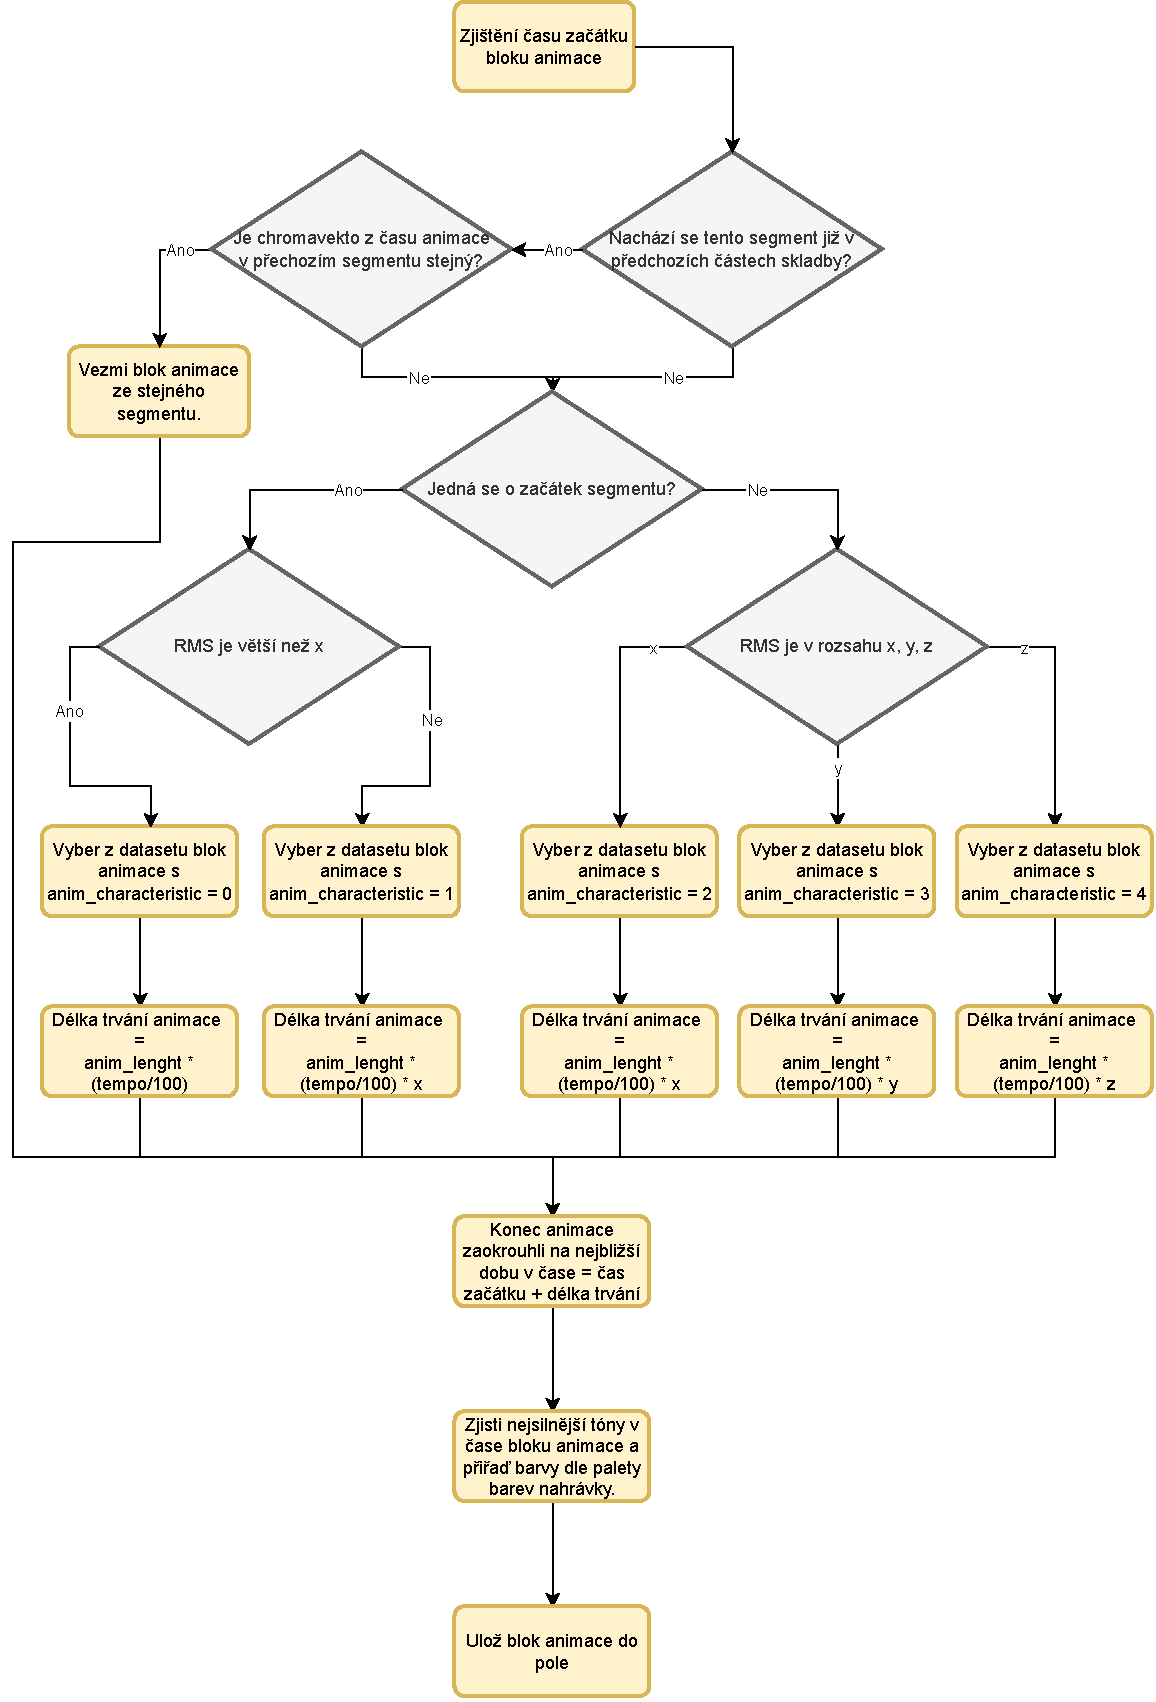
\includegraphics[width = 1\linewidth]{obrazky/Logical_structure_diagram.pdf}
    \caption{Struktura tříd }
    \label{fig:Logical_structure_diagram}
\end{figure}

% Na začátku je zjištěno jestli se jedná o první blok animace. Pokud ano je nastaven čas začátku animace jako čas první doby v nahrávce. Jestli se nejedná o první blok animace, tak je nastaven čas začátku jako konec předchozího bloku animace. Tento proces v blokovém schématu \ref{} představuje proces s názvem \uv{Nastavení času začátku animace}. Druhým krokem je rozhodovací struktura jestli se vybraný čas začátku nachází v segmentu nahrávky který se opakuje. Pokud ano je nalezen blok animace ve stejném času předchozího segmentu a je zkontrolováno  


\subsection{Databáze bloků animací} \label{sec:Database_structure}
Jak je popsáno v bodě \ref{sec:Spectoda}... jsou základní animace které jsou skládány dosebe a tak je možné vytvořit komplexní animace. Systém využívá již předsložených komplexních animací do bloků animací. Těmto blokům jsou přiřazeny parametry $code$, $characteristic$ a $length$ a jsou uloženy jako objekt datové třídy $AnimationBlock$.

Z objektů tipu $AnimationBlock$ jsou dále tvořeny datasety zapsané datovou třídou $Dataset$. Tyto datasety obsahují 5 bloků animací a parametry $genre$, $speed_suitability$ a $mood_characteristic$. UML diagramy těchto tříd jsou zobrazeny na obrázku \ref{fig:UML_diagram_Dataset_AnimationBlock}.

\begin{figure}[H]
    \centering
    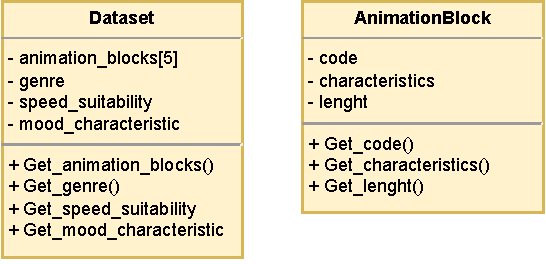
\includegraphics[width = 0.7\linewidth]{obrazky/UML_diagram_Dataset_and_AnimationBlock.pdf}
    \caption{Blokové diagramy tříd $Dataset$, $AnimationBlock$}
    \label{fig:UML_diagram_Dataset_AnimationBlock}
\end{figure}

\section{Výběr vhodných metod pro extrakci vlastností hudební nahrávky} \label{sec:Exktrakce_vlastnosti_metody}

Vědeská komunita nabízí několik volně šířících knihoven obsahující techniky z oborů MIR. V této části práce jsou prozkoumány 3 knihovny zmíněné v bodě \ref{sec:Dostupna_reseni}. Jsou použity jejich funkce získání potřebných parametrů hudební nahrávky potřebných pro navazující diplomovou práci. Tyto funkce jsou mezi sebou porovnány z hlediska přesnosti výsledků, rychlosti výpočtů, jednoduchosti použití a možnosti využití pro komerční účely. 

\subsection{Detekce dob a tempa}

\subsection{Analýza chromavektorů}

\subsection{Efektivní hodnota signálu}


Vstupními parametry systému jsou získané parametry jež jsou popsány v bodě \ref{sec:Parametry_nahravky} 

% Možná lepší první popsat strukturu systému jak by se měly animace generovat a co k tomu budou potřeba za parametry. Následně teprve vytvořit sekci kde je popsán vzniklý kód pro analýzu jednotlivých parametrů. Také důležité jestli ukázaky kódu atd.. nebudou zahrnuty spíše v sekci Věběr vhodných metod pro extrakci vlastností hudební nahrávky. 